\section{Transformator}


\begin{enumerate}

\item Transformator qanday asbob?
\begin{enumerate}[label=\Alph*)]
\item O‘zgaruvchan kuchlanishni kuchaytirib yoki pasaytirib beruvchi.
\item Zarrachalarni tezlashtiruvchi.
\item Elektromagnit tebranishlarni hosil qiluvchi.
\item Radioaktiv nurlanishlarni aniqlovchi.
\end{enumerate}


\item Transformatorning transformatsiya koeffitsienti ifodasini toping.
\begin{enumerate}[label=\Alph*)]
\item $k = \frac{U_1}{U_2}$.
\item $k = \frac{M}{q}$.
\item $k = \frac{F}{x}$.
\item $k = \frac{A}{zF}$.
\end{enumerate}

\item Transformatorning birinchi o‘ramidagi o‘ramlar soni 800 ta, ikkinchisidagi o‘ramlar soni 3200 ta. Transformatsiya koeffitsentini aniqlang.
\begin{enumerate}[label=\Alph*)]
\item 1/2.
\item 1/4.
\item 2.
\item 4.
\end{enumerate}

\item Transformatorning birinchi chulg‘amiga 220 V kuchlanish berildi. Agar transformatsiyalash koeffitsienti 0,8 bo‘lsa, ikkinchi chulg‘amdagi kuchlanish qanday bo‘ladi (V)?
\begin{enumerate}[label=\Alph*)]
\item 364.
\item 275.
\item 220.
\item 176.
\end{enumerate}

\item Transformatorning birlamchi chulg‘amiga 220 V kuchlanish berilgan. Birlamchi chulg‘amdagi o‘ramlar soni 400. Ikkilamchi chulg‘amdagi o‘ramlar soni 200. Ikkilamchi chulg‘amdagi kuchlanish qanday (V)?
\begin{enumerate}[label=\Alph*)]
\item 110.
\item 100.
\item 200.
\item 220.
\end{enumerate}

\item Transformatorning ikkilamchi chulg‘amidagi o‘ramlar soni 990 ta, kirishidagi kuchlanish 220 V, chiqishidagi kuchlanish 330 V bo‘lsa, birlamchi chulg‘amdagi o‘ramlar soni qanday?
\begin{enumerate}[label=\Alph*)]
\item 110.
\item 220.
\item 330.
\item 660.
\end{enumerate}

\item Transformatorning birlamchi chulg‘ami 40 o‘ramdan iborat. Kuchlanishni 220 V dan 22000 V gacha orttirish uchun transformatorning ikkilamchi chulg‘amidagi o‘ramlar soni nechta bo‘lishi kerak?
\begin{enumerate}[label=\Alph*)]
\item 22000.
\item 4000.
\item 2200.
\item 400.
\end{enumerate}


\item Quyidagi bir-biriga ulangan ideal transformatorlarda $N_1/N_2 = 8$ va $N_3/N_4 = 1/3$ bo‘lsa, chiqishdagi kuchlanish $U_2$ nimaga teng (V)?

\begin{center}
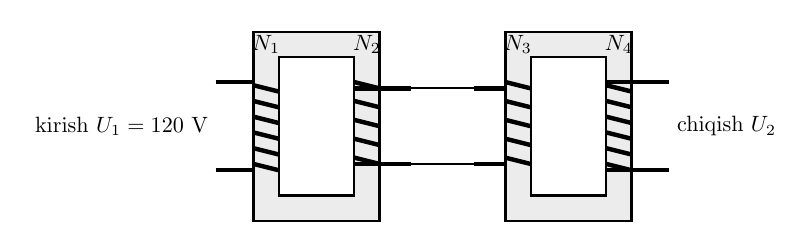
\begin{tikzpicture}[scale=0.8, every node/.style={transform shape}]
  % Birinchi o'zak (T1)
  \draw[thick, fill=gray!15] (0,0) rectangle (2,3);
  \draw[thick, fill=white] (0.4,0.4) rectangle (1.6,2.6);

  % Ikkinchi o'zak (T2)
  \draw[thick, fill=gray!15] (4,0) rectangle (6,3);
  \draw[thick, fill=white] (4.4,0.4) rectangle (5.6,2.6);

  % Chap chulg'am N1
  \draw[ultra thick] (-0.6, 2.2) -- (0, 2.2);
  \draw[ultra thick] (-0.6, 0.8) -- (0, 0.8);
  \foreach \y in {0.9, 1.15, 1.4, 1.65, 1.9, 2.15} {
    \draw[ultra thick] (0, \y) -- (0.4, \y-0.1);
  }
  \node at (0.2, 2.8) {$N_1$};
  \node[left] at (-0.6, 1.5) {kirish $U_1=120$~V};

  % O'ng chulg'am N2
  \draw[ultra thick] (1.6, 2.1) -- (2.5, 2.1);
  \draw[ultra thick] (1.6, 0.9) -- (2.5, 0.9);
  \foreach \y in {1.0, 1.3, 1.6, 1.9, 2.2} {
    \draw[ultra thick] (1.6, \y) -- (2, \y-0.1);
  }
  \node at (1.8, 2.8) {$N_2$};

  % O'tish simlari
  \draw[thick] (2.5, 2.1) -- (3.5, 2.1);
  \draw[thick] (2.5, 0.9) -- (3.5, 0.9);

  % T2 chap chulg'am N3
  \draw[ultra thick] (3.5, 2.1) -- (4, 2.1);
  \draw[ultra thick] (3.5, 0.9) -- (4, 0.9);
  \foreach \y in {1.0, 1.3, 1.6, 1.9, 2.2} {
    \draw[ultra thick] (4, \y) -- (4.4, \y-0.1);
  }
  \node at (4.2, 2.8) {$N_3$};

  % T2 o'ng chulg'am N4
  \draw[ultra thick] (5.6, 2.2) -- (6.6, 2.2);
  \draw[ultra thick] (5.6, 0.8) -- (6.6, 0.8);
  \foreach \y in {0.9, 1.15, 1.4, 1.65, 1.9, 2.15} {
    \draw[ultra thick] (5.6, \y) -- (6, \y-0.1);
  }
  \node at (5.8, 2.8) {$N_4$};
  \node[right] at (6.6, 1.5) {chiqish $U_2$};
\end{tikzpicture}
\end{center}

\begin{enumerate}[label=\Alph*)]
\item 15.
\item 30.
\item 45.
\item 60.
\end{enumerate}

\item Pasaytiruvchi transformatorning ikkilamchi chulg‘ami zanjiridagi kuchlanish 80 V va tok kuchi 2 A. Kuchlanish 160 V bo‘lgan birlamchi chulg‘amdagi tok kuchi necha Amper? Isrofni hisobga olmang.
\begin{enumerate}[label=\Alph*)]
\item 1.
\item 0,5.
\item 1,5.
\item 2.
\end{enumerate}

\item Ushbu transformatorda kirishdagi quvvat $P_1 = 100$ W, chiqishdagi quvvat $P_2 = 80$ W. $U_1/U_2 = 10$ bo‘lsa, $I_2/I_1$ nisbat nimaga teng?

\begin{center}
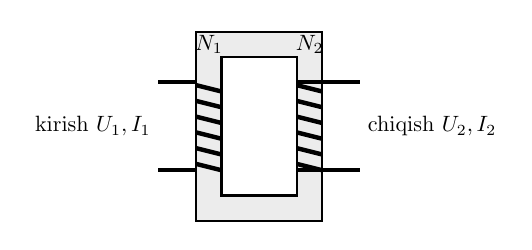
\begin{tikzpicture}[scale=0.8, every node/.style={transform shape}]
  % Transformator o'zagi
  \draw[thick, fill=gray!15] (0,0) rectangle (2,3);
  \draw[thick, fill=white] (0.4,0.4) rectangle (1.6,2.6);

  % Birlamchi chulg'am N1
  \draw[ultra thick] (-0.6, 2.2) -- (0, 2.2);
  \draw[ultra thick] (-0.6, 0.8) -- (0, 0.8);
  \foreach \y in {0.9, 1.15, 1.4, 1.65, 1.9, 2.15} {
    \draw[ultra thick] (0, \y) -- (0.4, \y-0.1);
  }
  \node at (0.2, 2.8) {$N_1$};
  \node[left] at (-0.6, 1.5) {kirish $U_1, I_1$};

  % Ikkilamchi chulg'am N2
  \draw[ultra thick] (1.6, 2.2) -- (2.6, 2.2);
  \draw[ultra thick] (1.6, 0.8) -- (2.6, 0.8);
  \foreach \y in {0.9, 1.15, 1.4, 1.65, 1.9, 2.15} {
    \draw[ultra thick] (1.6, \y) -- (2, \y-0.1);
  }
  \node at (1.8, 2.8) {$N_2$};
  \node[right] at (2.6, 1.5) {chiqish $U_2, I_2$};
\end{tikzpicture}
\end{center}

\begin{enumerate}[label=\Alph*)]
\item 1/8.
\item 1/6.
\item 4.
\item 8.
\end{enumerate}

\item FIK 90 \% bo‘lgan pasaytiruvchi transformator tarmoqdan 2600 W quvvat iste’mol qiladi. Ikkinchi chulg‘amdagi tok quvvatini aniqlang (kW).
\begin{enumerate}[label=\Alph*)]
\item 2,34.
\item 1,2.
\item 0,24.
\item 3,36.
\end{enumerate}

\item Transformatorning birlamchi chulg‘amidagi kuchlanish 200 V, tok kuchi 0,5 A, ikkinchi chulg‘amida 38 V va 2,5 A bo‘lsa, transformatorning FIK necha foiz?
\begin{enumerate}[label=\Alph*)]
\item 70.
\item 76.
\item 80.
\item 95.
\end{enumerate}

\item FIK i 75 \% bo‘lgan rasmdagi transformatorda birlamchi chulg‘amdagi tok kuchining effektiv qiymati $I_1 = 1$ A, kuchlanishning effektiv qiymati $U_1 = 200$ V. Ikkilamchi chulg‘amdagi $R = 6\ \Omega$ qarshilikdan o‘tayotgan tok kuchining effektiv qiymatini aniqlang (A).

\begin{center}
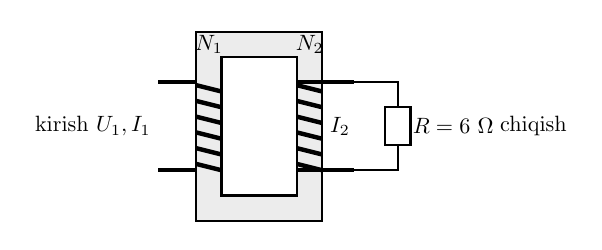
\begin{tikzpicture}[scale=0.8, every node/.style={transform shape}]
  % O'zak
  \draw[thick, fill=gray!15] (0,0) rectangle (2,3);
  \draw[thick, fill=white] (0.4,0.4) rectangle (1.6,2.6);

  % Birlamchi chulg'am N1
  \draw[ultra thick] (-0.6, 2.2) -- (0, 2.2);
  \draw[ultra thick] (-0.6, 0.8) -- (0, 0.8);
  \foreach \y in {0.9, 1.15, 1.4, 1.65, 1.9, 2.15} {
    \draw[ultra thick] (0, \y) -- (0.4, \y-0.1);
  }
  \node at (0.2, 2.8) {$N_1$};
  \node[left] at (-0.6, 1.5) {kirish $U_1, I_1$};

  % Ikkilamchi chulg'am N2
  \draw[ultra thick] (1.6, 2.2) -- (2.5, 2.2);
  \draw[ultra thick] (1.6, 0.8) -- (2.5, 0.8);
  \foreach \y in {0.9, 1.15, 1.4, 1.65, 1.9, 2.15} {
    \draw[ultra thick] (1.6, \y) -- (2, \y-0.1);
  }
  \node at (1.8, 2.8) {$N_2$};

  % R Qarshilik yuklamasi
  \draw[thick] (2.5, 2.2) -- (3.2, 2.2) -- (3.2, 1.8);
  \draw[thick] (3.0, 1.8) rectangle (3.4, 1.2) node[midway, right=3pt] {$R=6\ \Omega$};
  \draw[thick] (3.2, 1.2) -- (3.2, 0.8) -- (2.5, 0.8);
  \node[right] at (2.0, 1.5) {$I_2$};
  \node[right] at (4.7, 1.5) {chiqish};
\end{tikzpicture}
\end{center}

\begin{enumerate}[label=\Alph*)]
\item 5.
\item 4.
\item 3.
\item 2.
\end{enumerate}


\item Pasaytiruvchi transformator chiqishidagi kuchlanish 30 V. Unga har biri 0,8 A tok iste’mol qiladigan 100 ta lampochka ulangan. Agar transformatorning FIK 96\% bo‘lsa, uning kirishidagi quvvati qanday (kW)?
\begin{enumerate}[label=\Alph*)]
\item 1,5.
\item 2.
\item 4.
\item 2,5.
\end{enumerate}

\item Quvvati 60 kW, kuchlanishi 2400 V bo‘lgan generatordan energiya uzatishda liniyadagi kuchlanishning tushuvi 10\% dan oshmasligi uchun simlarning qarshiligi ko‘pi bilan necha $\Omega$ bo‘lishi kerak?
\begin{enumerate}[label=\Alph*)]
\item 60.
\item 48.
\item 24.
\item 9,6.
\end{enumerate}

\item 100 kW quvvatli elektr energiyani 10 kV kuchlanish bilan $17\text{ mm}^2$ ko‘ndalang kesimga ega bo‘lgan mis sim orqali uzatish kerak. Energiya sarfi 5\% dan oshib ketmasligi uchun uni qanday maksimal masofagacha uzatish mumkin (km)? $\rho = 1,7 \cdot 10^{-8}\ \Omega\cdot\text{m}$.
\begin{enumerate}[label=\Alph*)]
\item 5.
\item 10.
\item 25.
\item 20.
\end{enumerate}

\item Elektr uzatish tizimida kuchlanish 2 marta orttirilsa, uzatish simlarida ajralayotgan issiqlik miqdori qanday o‘zgaradi?
\begin{enumerate}[label=\Alph*)]
\item O‘zgarmaydi.
\item 4 marta ortadi.
\item 4 marta kamayadi.
\item 2 marta ortadi.
\end{enumerate}

\item Tok manbaining quvvatini o‘zgartirmagan holda kuchlanish oshirilganda, uzatish simlaridagi energiya isrofi 100 marta kamaygan. Kuchlanish necha marta oshirilgan?
\begin{enumerate}[label=\Alph*)]
\item 5.
\item 10.
\item 20.
\item 100.
\end{enumerate}

\end{enumerate}



\begin{table}[!ht]
\centering
\begin{tabular}{|c|c|c|c|c|c|c|c|c|c|c|}
\hline
1a & 2a & 3b & 4b & 5a & 6d & 7b & 8c & 9a & 10d & 11a \\ \hline
12d & 13a & 14d & 15d & 16c & 17c & 18b & & & & \\ \hline
\end{tabular}
\end{table}











\section{Elektromagnit To`lqinlar}

\begin{enumerate}

\item Quyidagi to‘lqinlarning qaysi biri bo‘ylama to‘lqin?
1) suv sirtidagi to‘lqinlar; 2) suyuqlik va gazlardagi tovush to‘lqinlari; 3) elektromagnit to‘lqinlar; 4) cholg‘u torlarida paydo bo‘luvchi to‘lqinlar.
\begin{enumerate}[label=\Alph*)]
\item 1.
\item 2.
\item 3.
\item 1 va 2.
\end{enumerate}

\item Elektromagnit to‘lqinlar qanday sharoitda nurlanadi?
\begin{enumerate}[label=\Alph*)]
\item zaryad tebranganda.
\item elektron to‘g‘ri chiziqli tekis harakatlanganda.
\item o‘tkazgichda elektron to‘g‘ri chiziqli tekis harakatda.
\item neytral atom tezlanish bilan harakatlanganda.
\end{enumerate}

\item 1-zaryad tekis va to‘g‘ri chiziqli harakatlanadi; 2-zaryad to‘g‘ri chiziqli tezlanuvchan harakatlanadi; 3-zaryad garmonik tebranishlar bajaradi; 4-zaryad aylana bo‘ylab tekis harakatlanadi. Bu zaryadlarning qaysilari elektromagnit to‘lqin nurlaydi?
\begin{enumerate}[label=\Alph*)]
\item faqat 1.
\item faqat 2.
\item 2, 3 va 4.
\item 1 va 2.
\end{enumerate}

\item Elektromagnit to‘lqinlar to‘lqinning qaysi turiga kiradi?
\begin{enumerate}[label=\Alph*)]
\item bo‘ylama.
\item bo‘ylama va ko‘ndalang.
\item ko‘ndalang.
\item bo‘ylama ham, ko‘ndalang ham emas.
\end{enumerate}

\item Elektromagnit to‘lqinlarning tarqalish yo‘nalishi qanday aniqlanadi? (Parmaning harakat yo‘nalishi qanday bo‘lsa, elektromagnit to‘lqinning tarqalish yo‘nalishi ham shunday bo‘ladi)
\begin{enumerate}[label=\Alph*)]
\item parmaning dastasi $\vec{E}$ dan $\vec{B}$ ga tomon aylantirilganda.
\item parmaning dastasi $\vec{B}$ dan $\vec{E}$ ga tomon aylantirilganda.
\item parmaning dastasi $\vec{E}$ dan soat mili yo‘nalishida aylantirilganda.
\item parmaning dastasi $\vec{E}$ dan soat mili harakatiga qarshi aylanganda.
\end{enumerate}

\item Manbadan tarqalayotgan elektromagnit to‘lqinning $\vec{E}$ va $\vec{B}$ vektorlari yo‘nalishi to‘lqin tarqalish yo‘nalishini ko‘rsatuvchi $\vec{v}$ vektor bilan qanday bog‘langan?
\begin{enumerate}[label=\Alph*)]
\item $\vec{E}\perp\vec{B}$; $\vec{E}$ va $\vec{v}$ parallel.
\item $\vec{E}\perp\vec{B}\perp\vec{v}$.
\item $\vec{E}\perp\vec{v}$; $\vec{E}$ va $\vec{B}$ parallel.
\item $\vec{B}\perp\vec{v}$; $\vec{E}$ va $\vec{v}$ parallel.
\end{enumerate}

\item Vakuumdagi $\vec{E}$ va $\vec{B}$ elektromagnit to‘lqin vektorlari X va Y o‘qlar bo‘ylab yo‘nalgan bo‘lsa, to‘lqinning tarqalish yo‘nalishi qanday?
\begin{enumerate}[label=\Alph*)]
\item X o‘qining musbat yo‘nalishida.
\item Y o‘qining musbat yo‘nalishida.
\item X o‘qining manfiy yo‘nalishida.
\item Z o‘qining musbat yo‘nalishida.
\end{enumerate}

\item Vakuumda elektromagnit to‘lqinlarning tarqalish tezligi...
\begin{enumerate}[label=\Alph*)]
\item muhitda tarqalish tezligiga teng bo‘ladi.
\item muhitda tarqalish tezligidan kichik bo‘ladi.
\item muhitda tarqalish tezligidan katta bo‘ladi.
\item nolga teng, chunki vakuumda umuman tarqalmaydi.
\end{enumerate}

\item Elektromagnit to‘lqinning 1- va 4- maksimumlari orasidagi masofa 30 m. Shu to‘lqinning uzunligi qanday (m)?
\begin{enumerate}[label=\Alph*)]
\item 30.
\item 15.
\item 10.
\item 7,5.
\end{enumerate}

\item Elektromagnit to‘lqinning chastotasi $\nu$, tezligi $v$ va to‘lqin uzunligi $\lambda$ orasidagi bog‘lanishni toping.
\begin{enumerate}[label=\Alph*)]
\item $\nu = \lambda/v$.
\item $\nu = v\lambda$.
\item $v = \lambda\nu$.
\item $v = \nu\lambda/2\pi$.
\end{enumerate}

\item Chastotasi $8\cdot 10^{14}$ Hz va to‘lqin uzunligi 200 nm bo‘lgan elektromagnit to‘lqinning tarqalish tezligi qanday (m/s)?
\begin{enumerate}[label=\Alph*)]
\item $4\cdot 10^7$.
\item $1,6\cdot 10^8$.
\item $2,5\cdot 10^7$.
\item $2\cdot 10^8$.
\end{enumerate}

\item Kosmik kemadan tarqalayotgan, chastotasi 10 MHz bo‘lgan elektromagnit to‘lqinning uzunligi qanday (m)?
\begin{enumerate}[label=\Alph*)]
\item 3.
\item 5.
\item 10.
\item 30.
\end{enumerate}

\item Vakuumda elektromagnit to‘lqin chastotasi $3\cdot 10^{13}$ Hz bo‘lsa, to‘lqin uzunligi qanday (m)?
\begin{enumerate}[label=\Alph*)]
\item $10^{-8}$.
\item $9\cdot 10^{13}$.
\item $0,01$.
\item $10^{-5}$.
\end{enumerate}

\item Chastotasi $8\cdot 10^{14}$ Hz va tarqalish tezligi $1,6\cdot 10^8$ m/s bo‘lgan elektromagnit to‘lqindagi rasmda ko‘rsatilgan masofani toping (nm).



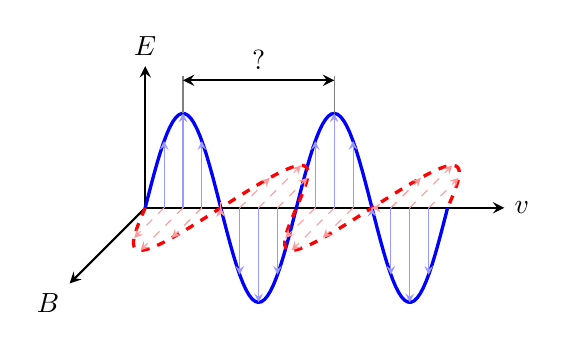
\begin{tikzpicture}[>=stealth, scale=1.2]
  % Koordinata o'qlari (E, B, v)
  \draw[->, thick] (0,0) -- (3.8,0) node[right] {$v$};
  \draw[->, thick] (0,0) -- (0,1.5) node[above] {$E$};
  \draw[->, thick] (0,0) -- (-0.8,-0.8) node[below left] {$B$};

  % E maydon to'lqini (sinusoida xy tekisligida - ko'k rangda)
  % To'lqin uzunligi lambda = 1.6 deb olindi. Ikkita to'liq tebranish: 3.2 gacha.
  \draw[very thick, blue] plot[domain=0:3.2, samples=100] (\x, {sin(\x * 360 / 1.6)});

  % B maydon to'lqini (sinusoida xz tekisligida, qiya proyeksiyada - qizil chiziqda)
  % Har bir x nuqta uchun siljish (-0.45*sin, -0.45*sin) ko'rinishida hosil qilinadi
  \draw[very thick, red, dashed] plot[domain=0:3.2, samples=100] 
    ({\x - 0.45*sin(\x * 360 / 1.6)}, {-0.45*sin(\x * 360 / 1.6)});

  % Kuch chiziqlari (E va B maydonlarining tebranish vektorlari)
  \foreach \x in {0.2, 0.4, 0.6, 0.8, 1.0, 1.2, 1.4, 1.8, 2.0, 2.2, 2.4, 2.6, 2.8, 3.0} {
    \pgfmathsetmacro{\val}{sin(\x * 360 / 1.6)}
    \draw[->, blue!40, thin] (\x, 0) -- (\x, \val);
    \draw[->, red!40, thin, dashed] (\x, 0) -- ({\x - 0.45*\val}, {-0.45*\val});
  }

  % Masofa ko'rsatkichi "?" (birinchi musbat maksimumdan ikkinchi musbat maksimumgacha)
  % Maksimumlar mos ravishda x = 0.4 va x = 2.0 nuqtalarda joylashgan (oraliq masofa = 1.6 = lambda)
  \draw[thin, gray] (0.4, 1.0) -- (0.4, 1.4);
  \draw[thin, gray] (2.0, 1.0) -- (2.0, 1.4);
  \draw[<->, thick] (0.4, 1.35) -- (2.0, 1.35) node[midway, above] {?};
\end{tikzpicture}


\begin{enumerate}[label=\Alph*)]
\item 500.
\item 400.
\item 320.
\item 200.
\end{enumerate}

\item ''Uyali`` telefon 100 MHz chastotada ishlaydi. Uning ishchi to‘lqin uzunligi qanday (m)?
\begin{enumerate}[label=\Alph*)]
\item 1.
\item 3.
\item 10.
\item 30.
\end{enumerate}

\item Elektromagnit to‘lqin dielektrik singdiruvchanligi $\varepsilon=2$ bo‘lgan muhitdan vakuumga o‘tdi. Bunda uning bir tebranish davriga teng vaqt davomidagi ko‘chish masofasi qanday o‘zgaradi?
\begin{enumerate}[label=\Alph*)]
\item avval ortadi, so‘ngra kamayadi.
\item ortadi.
\item o‘zgarmaydi.
\item kamayadi.
\end{enumerate}

\item Dielektrik singdiruvchanligi $\varepsilon$ va magnit singdiruvchanligi $\mu$ bo‘lgan muhitda tarqalayotgan elektromagnit to‘lqin tezligini hisoblash ifodasini ko‘rsating. Vakuumdagi tezlik – c, $\lambda_0$ va $\lambda$ lar mos ravishda vakuum va muhitdagi to‘lqin uzunliklari.
\begin{enumerate}[label=\Alph*)]
\item $c/\sqrt{\varepsilon\mu}$.
\item $c\sqrt{\varepsilon\mu}$.
\item $\sqrt{\varepsilon\mu}$.
\item $v/\lambda_0$.
\end{enumerate}

\item Elektromagnit to‘lqin intensivligi – bu ...
\begin{enumerate}[label=\Alph*)]
\item hajm birligidagi elektromagnit energiya W.
\item $\Delta S$ yuzadan $\Delta t$ vaqtda o‘tuvchi elektromagnit energiya W ning $\Delta S \Delta t$ ko‘paytmaga nisbati.
\item $\Delta S$ yuzadan o‘tuvchi elektromagnit energiya W ning $\Delta S$ kattalikka nisbati.
\item elektromagnit energiya W ning vaqt oralig‘i $\Delta t$ ga nisbati.
\end{enumerate}

\item Nuqtaviy manba elektromagnit nurlanishining intensivligi ...
\begin{enumerate}[label=\Alph*)]
\item manbadan bo‘lgan masofaga to‘g‘ri proporsional.
\item manbadan bo‘lgan masofaga teskari proporsional.
\item manbadan bo‘lgan masofa kvadratiga proporsional.
\item manbadan bo‘lgan masofa kvadratiga teskari proporsional.
\end{enumerate}

\item Elektromagnit nurlanish yo‘nalishi bo‘ylab birinchi nuqtadan ikkinchi nuqtaga 6 m ko‘chilganda nurlanish intensivligi 4 marta kamaygan. Birinchi nuqta nurlanish manbaidan qancha masofada (m) joylashgan?
\begin{enumerate}[label=\Alph*)]
\item 6.
\item 18.
\item 12.
\item 24.
\end{enumerate}

\item Ergacha bo‘lgan masofani $150\cdot 10^6$ km deb olib, Quyoshning to‘la nurlanish quvvatini toping (kW).
\begin{enumerate}[label=\Alph*)]
\item $1,5\cdot 10^{31}$.
\item $2\cdot 10^{29}$.
\item $3\cdot 10^{23}$.
\item $4\cdot 10^{23}$.
\end{enumerate}

\item Agar elektromagnit tebranishlar chastotasi 2 marta orttirilsa, ochiq tebranishlar konturidan nurlanadigan quvvat qanday o‘zgaradi?
\begin{enumerate}[label=\Alph*)]
\item o‘zgarmaydi.
\item 2 marta kamayadi.
\item 2 marta ortadi.
\item 16 marta ortadi.
\end{enumerate}

\item Agar vibratordan nurlanayotgan elektromagnit to‘lqin chastotasi 3 marta ortsa, vaqt birligida undan nurlanayotgan to‘lqin energiyasi necha marta ortadi? To‘lqin amplitudasini o‘zgarmas deb hisoblang.
\begin{enumerate}[label=\Alph*)]
\item 27.
\item 81.
\item 12.
\item 3.
\end{enumerate}

\end{enumerate}




\begin{table}[!ht]
\centering
\begin{tabular}{|c|c|c|c|c|c|c|c|c|c|c|}
\hline
1b & 2a & 3c & 4c & 5a & 6b & 7d & 8c & 9c & 10c & 11b \\ \hline
12d & 13d & 14d & 15b & 16b & 17a & 18b & 19d & 20a & 21d & 22d \\ \hline
23b & & & & & & & & & & \\ \hline
\end{tabular}
\end{table}













\section{Radioaloqa}

\begin{enumerate}

\item Radiopriyomnikning tebranish konturidagi tok kuchining o‘zgarish qonuni $i = 10^{-6}\sin10^6\pi t$ (A) ko‘rinishda bo‘lsa, u necha Hz chastotaga moslangan?
\begin{enumerate}[label=\Alph*)]
\item $10^5$.
\item $5\cdot 10^5$.
\item $10^6$.
\item $5\cdot 10^6$.
\end{enumerate}

\item Agar priyomnik tebranishlar konturining kondensatoridagi zaryadning o‘zgarish qonuni $q = 2 \cdot 10^{-9}\sin5 \cdot 10^5\pi t$ (C) ko‘rinishda bo‘lsa, qabul qilinayotgan to‘lqinning uzunligi qanday (m)?
\begin{enumerate}[label=\Alph*)]
\item 200.
\item 500.
\item 1000.
\item 1200.
\end{enumerate}

\item Agar radiopriyomnik konturining kondensatoridagi zaryad $q = 10^{-9}\cos4 \cdot 10^4\pi t$ (C) qonun bo‘yicha o‘zgarayotgan bo‘lsa, priyomnik qanday chastotaga moslangan (Hz)?
\begin{enumerate}[label=\Alph*)]
\item $5\cdot 10^5$.
\item $10^6\pi$.
\item $10^6$.
\item $2\cdot 10^4$.
\end{enumerate}

\item Radiopriyomnikning qabul qilish chastotasini 2 marta oshirish uchun uning tebranish konturidagi kondensator sig‘imini qanday o‘zgartirish kerak?
\begin{enumerate}[label=\Alph*)]
\item 2 marta oshirish.
\item 4 marta kamaytirish.
\item 4 marta oshirish.
\item 2 marta kamaytirish.
\end{enumerate}

\item Kosmik kemada o‘rnatilgan radiouzatgich 20 MHz chastotada ishlaydi. U nurlaydigan radioto‘lqinning uzunligi qanday (m)?
\begin{enumerate}[label=\Alph*)]
\item 10.
\item 15.
\item 30.
\item 100.
\end{enumerate}

\item Antenna 6 MHz chastotali elektromagnit to‘lqin nurlamoqda. To‘lqin tarqalish yo‘nalishidagi 100 km masofada nechta to‘lqin joylashadi?
\begin{enumerate}[label=\Alph*)]
\item 1000.
\item 1500.
\item 1800.
\item 2000.
\end{enumerate}

\item Konturda 5 MHz chastotali radioto‘lqin hosil bo‘lmoqda. To‘lqin tarqalish yo‘nalishidagi 150 km masofada nechta to‘lqin uzunligi joylashadi?
\begin{enumerate}[label=\Alph*)]
\item 2500.
\item 2000.
\item 1800.
\item 1500.
\end{enumerate}

\item To‘lqin uzunligi 10 cm bo‘lgan radioto‘lqinning chastotasini aniqlang (Hz).
\begin{enumerate}[label=\Alph*)]
\item $3,3\cdot 10^8$.
\item $3\cdot 10^7$.
\item $3\cdot 10^8$.
\item $3\cdot 10^9$.
\end{enumerate}

\setcounter{enumi}{8}
\item Radiopriyomnikning tebranish konturidagi kondensator sig‘imi 1000 pF, g‘altak induktivligi 1 mH bo‘lsa, u qanday (m) to‘lqin uzunlikka sozlangan bo‘ladi?
\begin{enumerate}[label=\Alph*)]
\item 628.
\item 942.
\item 1884.
\item 314.
\end{enumerate}

\item Radiopriyomnikdagi 300 m to‘lqin uzunligiga mos keladigan tebranishlar konturining induktivligi 2,5 mH bo‘lsa, konturdagi kondensator sig‘imi qanday (pF)? $\pi^2\approx 10$.
\begin{enumerate}[label=\Alph*)]
\item 5.
\item 10.
\item 25.
\item 30.
\end{enumerate}

\item Agar to‘lqin uzunligi 1884 m bo‘lgan radioto‘lqinga moslangan tebranish konturidagi induktivlik 2 mH bo‘lsa, undagi kondensator sig‘imi qanday (pF)?
\begin{enumerate}[label=\Alph*)]
\item 500.
\item 188,4.
\item 314.
\item 942.
\end{enumerate}

\item 1884 m to‘lqin uzunligiga moslangan tebranishlar konturidagi kondensator sig‘imi 500 pF bo‘lsa, undagi g‘altakning induktivligi qanday (mH)?
\begin{enumerate}[label=\Alph*)]
\item 2.
\item 20.
\item 100.
\item 200.
\end{enumerate}

\item Nurlantirilayotgan elektromagnit to‘lqinlari uzunligi $1,2\cdot 10^8$ m. Radio antennasidagi tokning o‘zgarish qonuni qanday?
\begin{enumerate}[label=\Alph*)]
\item $i = I\sin 15,7t$.
\item $i = I\sin 12t$.
\item $i = I\sin 2\pi t$.
\item $i = I\sin 31,47t$.
\end{enumerate}

\setcounter{enumi}{13}
\item Agar radiolokatordan yuborilgan signal 420 $\mu$s da qaytgan bo‘lsa, obektgacha bo‘lgan masofa qanday (km)?
\begin{enumerate}[label=\Alph*)]
\item 36,5.
\item 63.
\item 73.
\item 126.
\end{enumerate}

\item Agar radiolokator 1 s da 1000 ta impuls nurlasa, u ko‘pi bilan qanday masofadagi obektni kuzatishga mo‘ljallangan (km)?


\begin{enumerate}[label=\Alph*)]
\item 1000.
\item 500.
\item 300.
\item 150.
\end{enumerate}

\item Radiolokator 1 s da 2000 impuls yuboradi. Radiolokator mo‘ljallangan o‘lchash uzoqligini toping (km).
\begin{enumerate}[label=\Alph*)]
\item 30.
\item 150.
\item 75.
\item 300.
\end{enumerate}

\end{enumerate}




\begin{table}[!ht]
\centering
\begin{tabular}{|c|c|c|c|c|c|c|c|c|c|c|}
\hline
1b & 2d & 3d & 4b & 5b & 6d & 7a & 8d & 9c & 10b & 11a \\ \hline
12a & 13a & 14b & 15d & 16c & & & & & & \\ \hline
\end{tabular}
\end{table}